\begin{align}
\vec{D}&=\frac{\vec{B}+\vec{C}}{2}
=\myvec{\frac{7}{2}\\[2pt] \frac{9}{2}}\\
\vec{E}&=\frac{\vec{A}+\vec{C}}{2}
=\myvec{\frac{5}{2}\\ 3}\\
\vec{F}&=\frac{\vec{A}+\vec{B}}{2}
=\myvec{5\\ \frac{7}{2}}
\\
\vec{P}
	&=\vec{Q}
=\vec{R}
=\frac{1}{3}\myvec{11\\11}
\\
\vec{G}&=\frac{\vec{A}+\vec{B}+\vec{C}}{3}
=\frac{1}{3}\myvec{11\\11}
\end{align} 
is the centroid.
See 
  \figref{fig:chapters/10/7/4/7/Figure}.
\begin{figure}[h!]
\centering
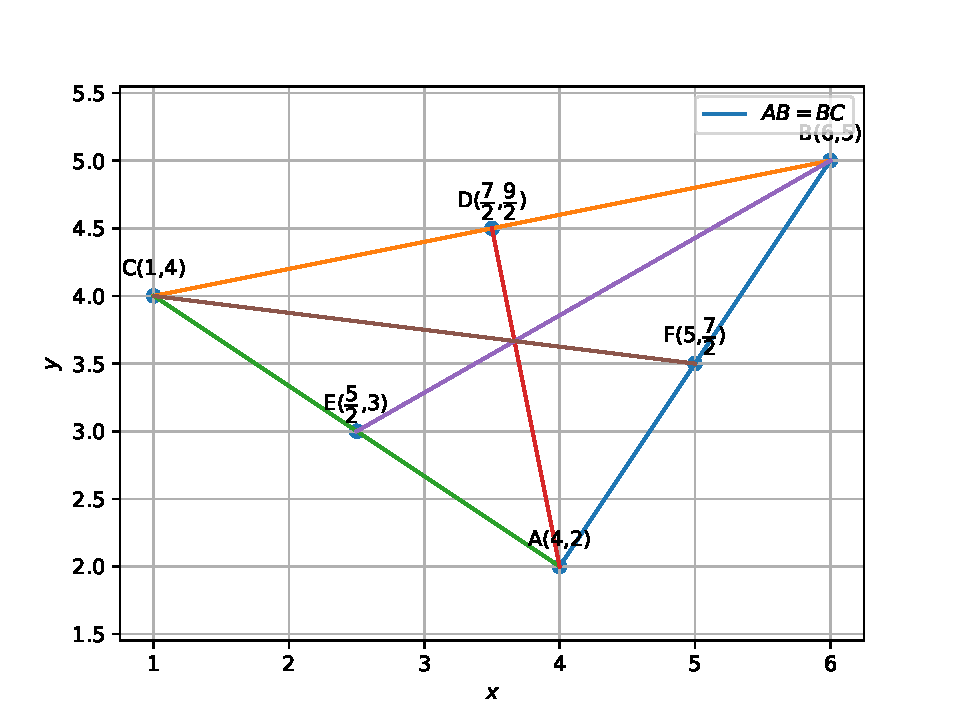
\includegraphics[width=\columnwidth]{chapters/10/7/4/7/figs/dj.pdf}
\caption{}
  \label{fig:chapters/10/7/4/7/Figure}
\end{figure}
